\subsection{Execution competence and decision uncertainty}
The primary run recorded 4,800 attempts, 4,783 valid choices, and 17 transport failures. Both returned model identifiers match their pinned requested snapshots. Failed records are retained as an observable category. No retries replace them.

Table~\ref{tab:model-performance} reports field-task performance, counting a failure as no delivered utility. Mini chooses a utility maximizer more often and incurs lower mean synthetic regret. These are descriptive results for the frozen generator, not a general model ranking. Calibration tasks are excluded from these field-performance denominators.

\begin{table}[t]
\centering\small
\begin{tabular}{@{}lrr@{}}
\toprule Field metric & Mini & Nano \\\midrule
Tasks & 1,440 & 1,440 \\
Utility-maximizing choice & 73.19\% & 55.69\% \\
Mean synthetic regret & 0.0186 & 0.0573 \\
Field delivery failures & 0.35\% & 0.28\% \\\bottomrule
\end{tabular}
\caption{Real model responses to constructed utility objectives. Regret is best available utility minus delivered utility, on the declared $[0,1]$ scale.}
\label{tab:model-performance}
\end{table}

The joint-mass diagnostic leaves all 18 conditions per model unresolved. It contains each known synthetic target, but this does not establish an empirical coverage rate: conditions share calibration data, and the set is small and selected. Zero wrong certified decisions is achieved here by abstaining on every condition. Even the optimal-choice control leaves all 18 corresponding intervals unresolved. At this budget, conservative coordinate boxes are not a practically sufficient product-selection procedure.

The constrained point baseline selects the wrong sign in 2 of 18 Mini conditions and 4 of 18 Nano conditions. The fixed-channel percentile bootstrap contains the known target in 14 of 18 and 16 of 18 conditions, respectively. These are descriptive counts, not a calibrated coverage comparison. The bootstrap omits calibration error; the conservative method includes it but sacrifices decisiveness. This experiment does not isolate intrinsic channel nonidentification from finite-sample uncertainty.

\begin{figure*}[t]
\centering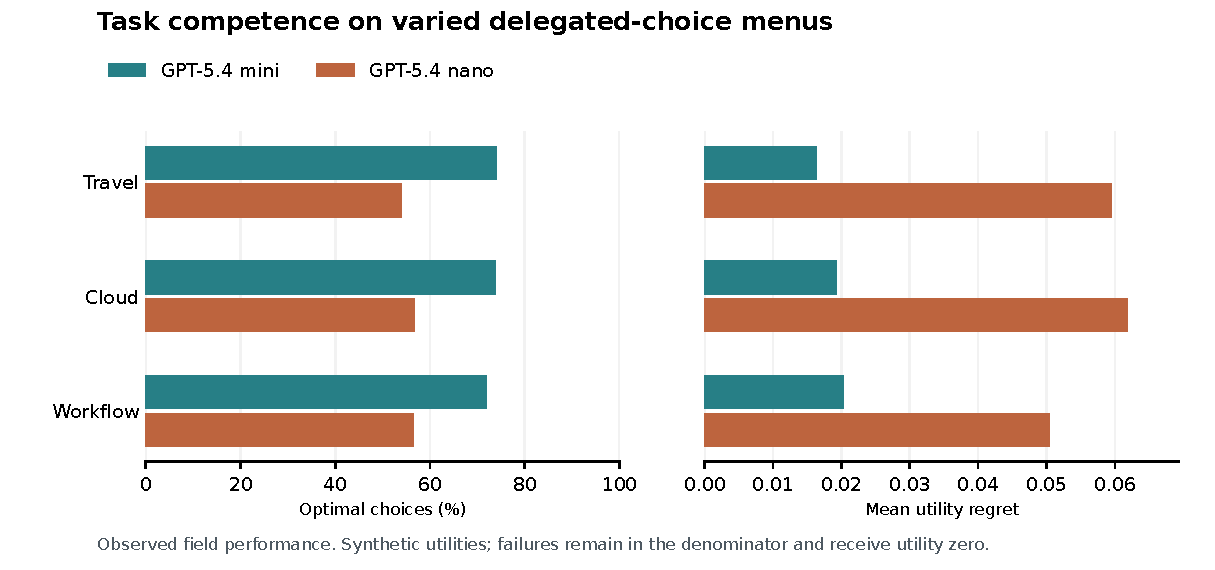
\includegraphics[width=.94\textwidth]{../results/model-study-summary/task-performance.pdf}
\caption{Primary field-task performance by semantic framing. The three framings share a mathematical generator. Real provider failures remain in the operational scores.}
\label{fig:performance}
\end{figure*}

\begin{figure*}[t]
\centering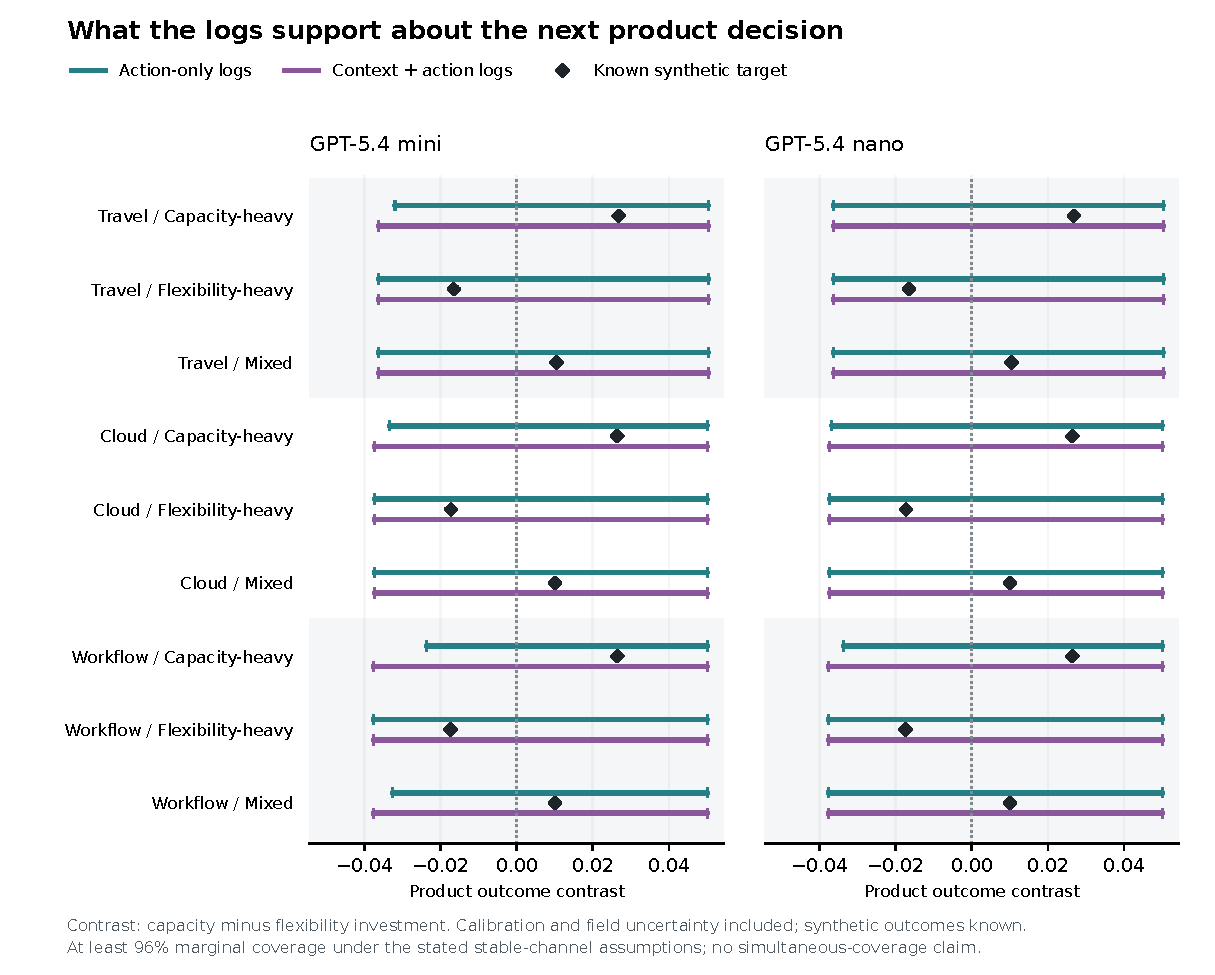
\includegraphics[width=.95\textwidth]{../results/model-study-summary/decision-intervals.pdf}
\caption{Primary decision intervals for the known finite-bank synthetic contrast. Each row uses the same independent calibration within a domain. Markers show the evaluation-only true target. All intervals cross zero. Nominal marginal coverage is at least 96\% under the stated model and sampling assumptions; this is not a simultaneous guarantee.}
\label{fig:intervals}
\end{figure*}

\subsection{Compute and interpretation}
Recorded tokens imply an estimated US\$1.113 for the primary run at the documented standard rates. This is not an invoice: failed transport requests may have unreported billable usage. Timeouts and connection resets are not evidence of model reasoning errors. Their temporal clustering also cautions against treating every operational error as an independent stationary draw. Conditional mathematical coverage statements must not be mistaken for verified provider independence.

The secondary analysis also propagates synthetic outcome estimation error and is more conservative. Exact outcome-bank values describe best attainable utility after future investment, not realized future behavior of the tested models. The primary findings justify investigating additional measurement channels, not declaring that all delegated product activity is inherently uninformative.
